\documentclass[11pt]{article}
\usepackage{amsmath,amssymb}
\usepackage{tikz}
\makeatletter
\newcommand\report[2]{%
  \pgfextracty{\dimen6}{\pgfpointdiff{\pgfpointanchor{#1}{center}}{\pgfpointanchor{#1}{north}}}%
  \pgfextracty{\dimen8}{\pgfpointdiff{\pgfpointanchor{#1}{south}}{\pgfpointanchor{#1}{center}}}%
  \typeout{GOT #2 N=\the\dimen6 S=\the\dimen8}}
\makeatother
\begin{document}
\begin{tikzpicture}
  \node (n0) at (0,0) {T};
  \report{n0}{0}
\end{tikzpicture}
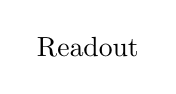
\begin{tikzpicture}
  \node (n1) at (0,0) {Readout};
  \report{n1}{1}
\end{tikzpicture}
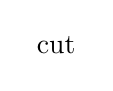
\begin{tikzpicture}
  \node (n2) at (0,0) {cut};
  \report{n2}{2}
\end{tikzpicture}
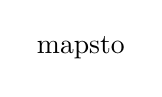
\begin{tikzpicture}
  \node (n3) at (0,0) {mapsto};
  \report{n3}{3}
\end{tikzpicture}
\begin{tikzpicture}
  \node (n4) at (0,0) {p_{\mathrm{good}}};
  \report{n4}{4}
\end{tikzpicture}
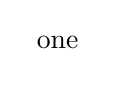
\begin{tikzpicture}
  \node (n5) at (0,0) {one\two};
  \report{n5}{5}
\end{tikzpicture}
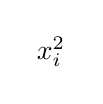
\begin{tikzpicture}
  \node (n6) at (0,0) {$x_i^2$};
  \report{n6}{6}
\end{tikzpicture}
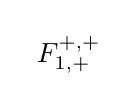
\begin{tikzpicture}
  \node (n7) at (0,0) {$F_{1,+}^{+,+}$};
  \report{n7}{7}
\end{tikzpicture}
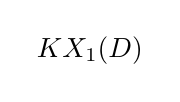
\begin{tikzpicture}
  \node (n8) at (0,0) {$KX_1(D)$};
  \report{n8}{8}
\end{tikzpicture}
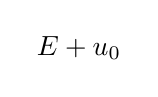
\begin{tikzpicture}
  \node (n9) at (0,0) {$E+u_0$};
  \report{n9}{9}
\end{tikzpicture}
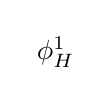
\begin{tikzpicture}
  \node (n10) at (0,0) {$\phi_H^1$};
  \report{n10}{10}
\end{tikzpicture}
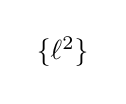
\begin{tikzpicture}
  \node (n11) at (0,0) {$\{\ell^2\}$};
  \report{n11}{11}
\end{tikzpicture}
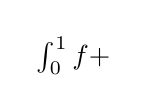
\begin{tikzpicture}
  \node (n12) at (0,0) {$\int_0^1 f$+};
  \report{n12}{12}
\end{tikzpicture}

\begin{tikzpicture}
  \node (n13) at (0,0) {Reset};
  \report{n13}{13}
\end{tikzpicture}
\end{document}
